% 圆锥曲线的光学性质
% 圆锥曲线|椭圆|抛物线|双曲线|角|光学性质

\pentry{椭圆的三种定义\upref{Elips3}, 抛物线的三种定义\upref{Para3}, 双曲线的三种定义\upref{Hypb3}}

首先,对于本词条涉及到的部分几何概念作出如下规定:
\begin{itemize}
\item \bb{角度}:所有角大小均取弧度制 $[0,\pi]$ 范围内的值(不区分始边终边,不区分正负角);
\item \bb{补角}:角的其中一条边的反向延长线与该角的另一条边所形成的角,称为该角的补角(如图1,$\angle A'BC$ 是 $\angle ABC$ 的补角,$\angle A'BC + \angle ABC = \pi$);
\begin{figure}[ht]
\centering
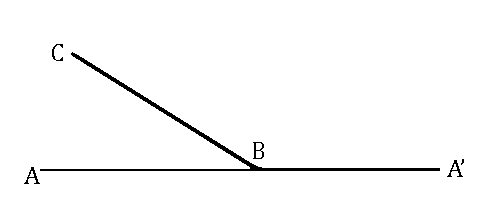
\includegraphics[width=8cm]{./figures/ConOpt1.pdf}
\caption{补角} \label{ConOpt_fig1}
\end{figure}
\item \bb{角平分线}:到角两边的距离相等的点的集合(把角分为大小相等的两部分的直线),称为该角的角平分线.
\end{itemize}
对两种特殊角的情形作出如下补充:
\begin{itemize}
\item 零角(如图2,$\angle ABC = 0$)的补角为平角($\angle ABA' = \pi$),零角的平分线与角两边重合(直线 $AA'$ 即 $\angle ABC$ 的平分线);
\item 平角(如图2,$\angle ABA' = \pi$)的补角为零角($\angle ABC = 0$),平角的平分线与角两边垂直($AA'$ 的垂线 $BN$ 即 $\angle ABA'$ 的平分线).
\end{itemize}
\begin{figure}[ht]
\centering
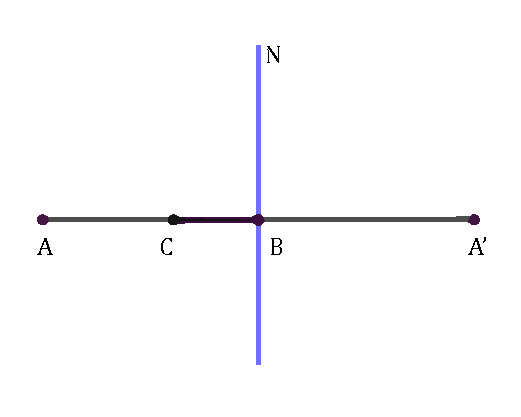
\includegraphics[width=8cm]{./figures/ConOpt2.pdf}
\caption{零角和平角} \label{ConOpt_fig2}
\end{figure}
显然,对所有角而言,\bb{角平分线与该角的补角平分线互相垂直}.

\subsection{椭圆的光学性质}
$F_1$,$F_2$ 是椭圆的两个焦点,$ P $ 是椭圆上任意一点,则 $\angle F_1PF_2 $ 的补角平分线 $ PT $ 是椭圆的切线.
\begin{figure}[ht]
\centering
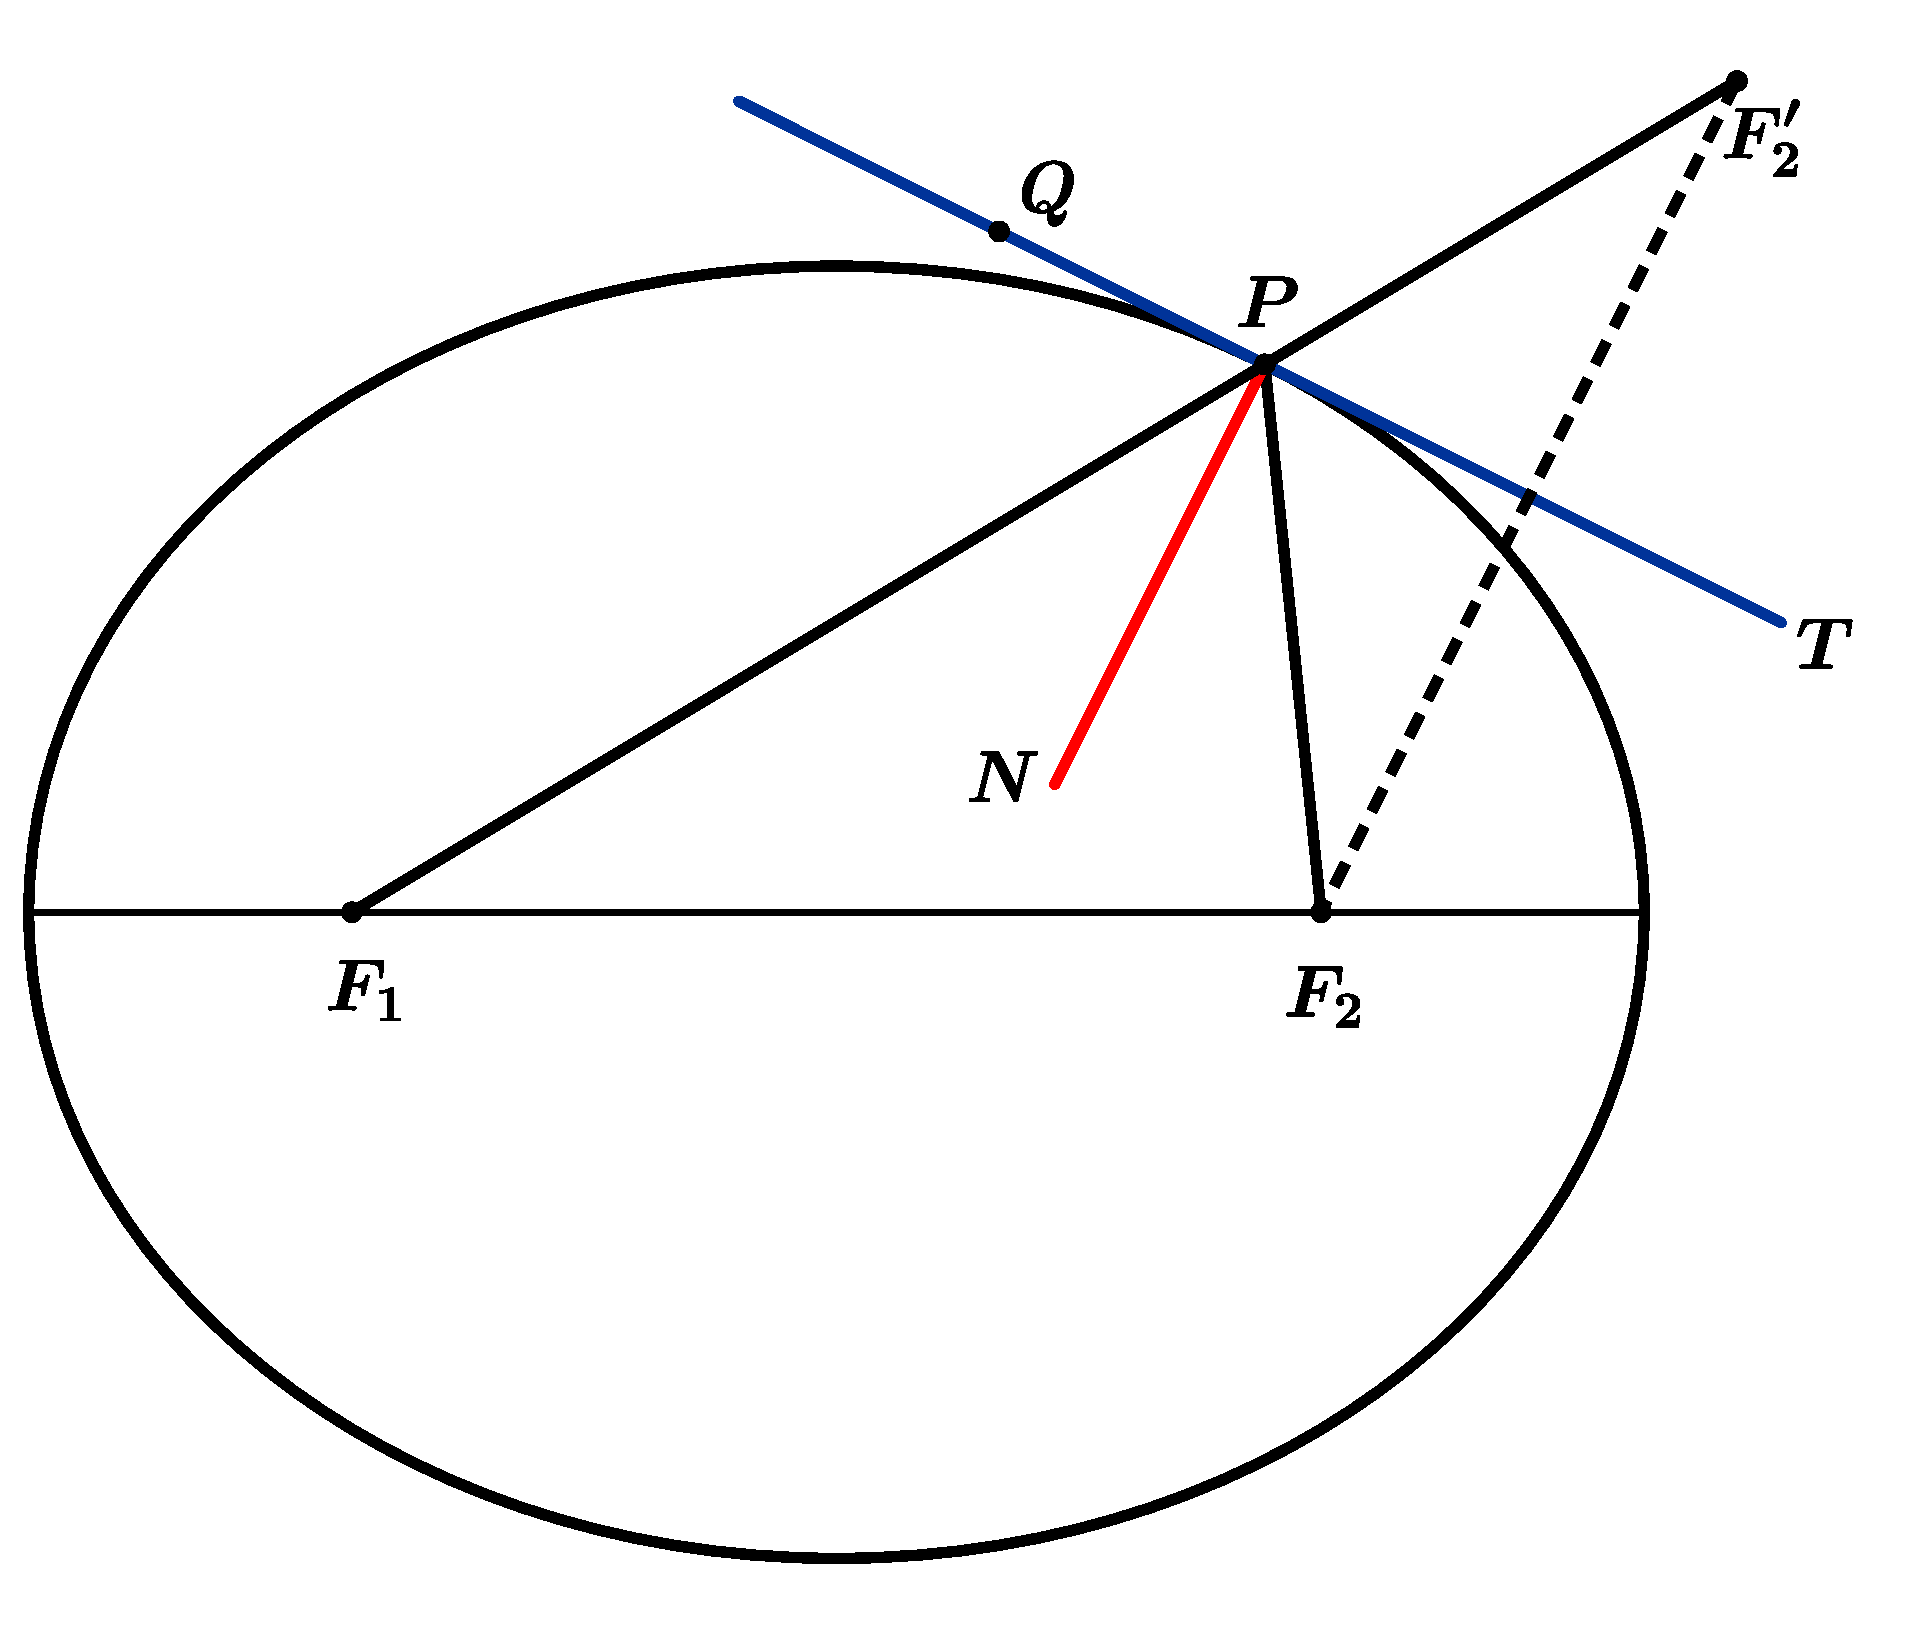
\includegraphics[width=8cm]{./figures/ConOpt3.pdf}
\caption{椭圆的光学性质} \label{ConOpt_fig3}
\end{figure}
\subsubsection{几何法证明}
作点 $F_2$ 关于直线 $PT$ 的对称点 $F_2'$.由于 $PT$ 是 $\angle F_1PF_2 $ 的补角平分线,则 $F_2'$ 在 $F_1P$ 的延长线上.

记 $Q$ 是直线 $PT$ 上的任意一点.于是
\begin{equation}\label{ConOpt_eq1}
F_1Q + F_2Q = F_1Q + F_2'Q \ges F_1F_2' = F_1P + F_2P
\end{equation}
当且仅当 $P$,$Q$ 重合时,不等式(\autoref{ConOpt_eq1})为等式.

椭圆的一种定义\upref{Elips3}为:
平面上到两焦点的距离之和为定值的点的集合. 显然, 椭圆内任意一点到两焦点距离之和小于该定值, 而椭圆外任意一点到两焦点距离之和大于该定值. 

所以, 直线 $PT$ 上有且仅有点 $P$ 在椭圆上, 其他点都在椭圆外. 这就证明了 $PT$ 是椭圆的切线.

\subsubsection{等价的命题}
结合光在同一介质中直线传播的性质,以及光的反射定律 —— 反射角等于入射角,不难推知,上述几何命题等价于物理命题“真空或同种均匀介质中,从椭圆一个焦点处射出的光线经过在椭圆曲线上的反射后,反射光线都汇聚于另一个焦点”.

\subsubsection{解析法推导}
记椭圆的直角坐标方程为
\begin{equation}\label{ConOpt_eq2}
b^2 x^2 +a^2 y^2=a^2 b^2
\end{equation}
其中 $a>b>0,c>0$ 且 $c^2=a^2-b^2$,椭圆焦距为 $2c$.

将 $y$ 视作 $x$ 的函数,对方程\autoref{ConOpt_eq2} 等号两边关于 $x$ 求导,可得
\begin{equation}
b^2 x +a^2 yy'= 0
\end{equation}

$P(x_0,y_0)$ 是椭圆上任意一点,则点 $P$ 处的椭圆切线方程为
\begin{equation}
a^2 y_0 \qty(y - y_0) = - b^2 x_0 \qty(x - x_0) \quad
\Rightarrow \quad
b^2 x_0 x + a^2 y_0 y = a^2 b^2
\end{equation}

由切线方程可得椭圆在点 $P$ 处的一个法向量(与切线垂直的向量)为 $\vec n = \qty(b^2 x_0,a^2 y_0)$.

向量 $\overrightarrow{F_1P}=\qty(x_0 +c,y_0)\; ,\; \overrightarrow{F_2P}=\qty(x_0 -c,y_0)$.

记两个任意向量($\vec s$ 和 $\vec t$)的夹角为 $<\vec s,\vec t>$.则
\begin{equation}\label{ConOpt_eq5}
\cos<\vec n,\overrightarrow{F_1P}>=\frac{\vec n \vdot \overrightarrow{F_1P}}{|\vec n| \; |\overrightarrow{F_1P}|}= \frac{b^2 x_0 (x_0+c)+a^2 y_0^2}{\sqrt{b^4 x_0^2+a^4 y_0^2}\sqrt{(x_0+c)^2+y_0^2}}
\end{equation}
\begin{equation}\label{ConOpt_eq6}
\cos<\vec n,\overrightarrow{F_2P}>=\frac{\vec n \vdot \overrightarrow{F_2P}}{|\vec n| \; |\overrightarrow{F_2P}|}= \frac{b^2 x_0 (x_0-c)+a^2 y_0^2}{\sqrt{b^4 x_0^2+a^4 y_0^2}\sqrt{(x_0-c)^2+y_0^2}}
\end{equation}

\autoref{ConOpt_eq5} 和\autoref{ConOpt_eq6} 作比,并代入\autoref{ConOpt_eq2} 及 $c^2=a^2-b^2$ 进行化简
\begin{equation}
\begin{aligned}
\frac{\cos<\vec n,\overrightarrow{F_1P}>}{\cos<\vec n,\overrightarrow{F_2P}>} &=\frac{a^2 b^2+b^2cx_0}{a^2 b^2-b^2cx_0}\; \sqrt{\frac{(x_0-c)^2+y_0^2}{(x_0+c)^2+y_0^2}} \\
&=\frac{a^2+cx_0}{a^2-cx_0}\; \sqrt{\frac{a^2(x_0-c)^2 +a^2 b^2-b^2 x_0^2}{a^2(x_0+c)^2 +a^2 b^2-b^2 x_0^2}} \\
&=\frac{a^2+cx_0}{a^2-cx_0}\; \sqrt{\frac{c^2 x_0^2 + a^4 - 2a^2 c x_0}{c^2 x_0^2 + a^4 + 2a^2 c x_0}} \\
&=\frac{a^2+cx_0}{a^2-cx_0}\; \sqrt{\frac{(a^2-cx_0)^2}{(a^2+cx_0)^2}}
\end{aligned}
\end{equation}

由于点 $P$ 在椭圆上,则 $-a\les x_0 \les a$,则 $a^2-cx_0 >0$,因此
\begin{equation}
\frac{\cos<\vec n,\overrightarrow{F_1P}>}{\cos<\vec n,\overrightarrow{F_2P}>}=1
\end{equation}

所以 $<\vec n,\overrightarrow{F_1P}>=<\vec n,\overrightarrow{F_2P}>$,满足入射角等于反射角的反射定律.由此用解析几何的方法推导出了椭圆的光学性质.


\subsection{抛物线的光学性质}
$F$ 是抛物线的焦点,$l$ 是准线,$P$ 是抛物线上的任意一点,作 $PP' \perp l$,垂足为 $P'$,则 $\angle FPP' $ 的角平分线 $ PT $ 是抛物线的切线.

等价命题:真空或同种均匀介质中,从抛物线焦点射出的光线,经过抛物线曲线的反射后,反射光线平行于抛物线对称轴.
\begin{figure}[ht]
\centering
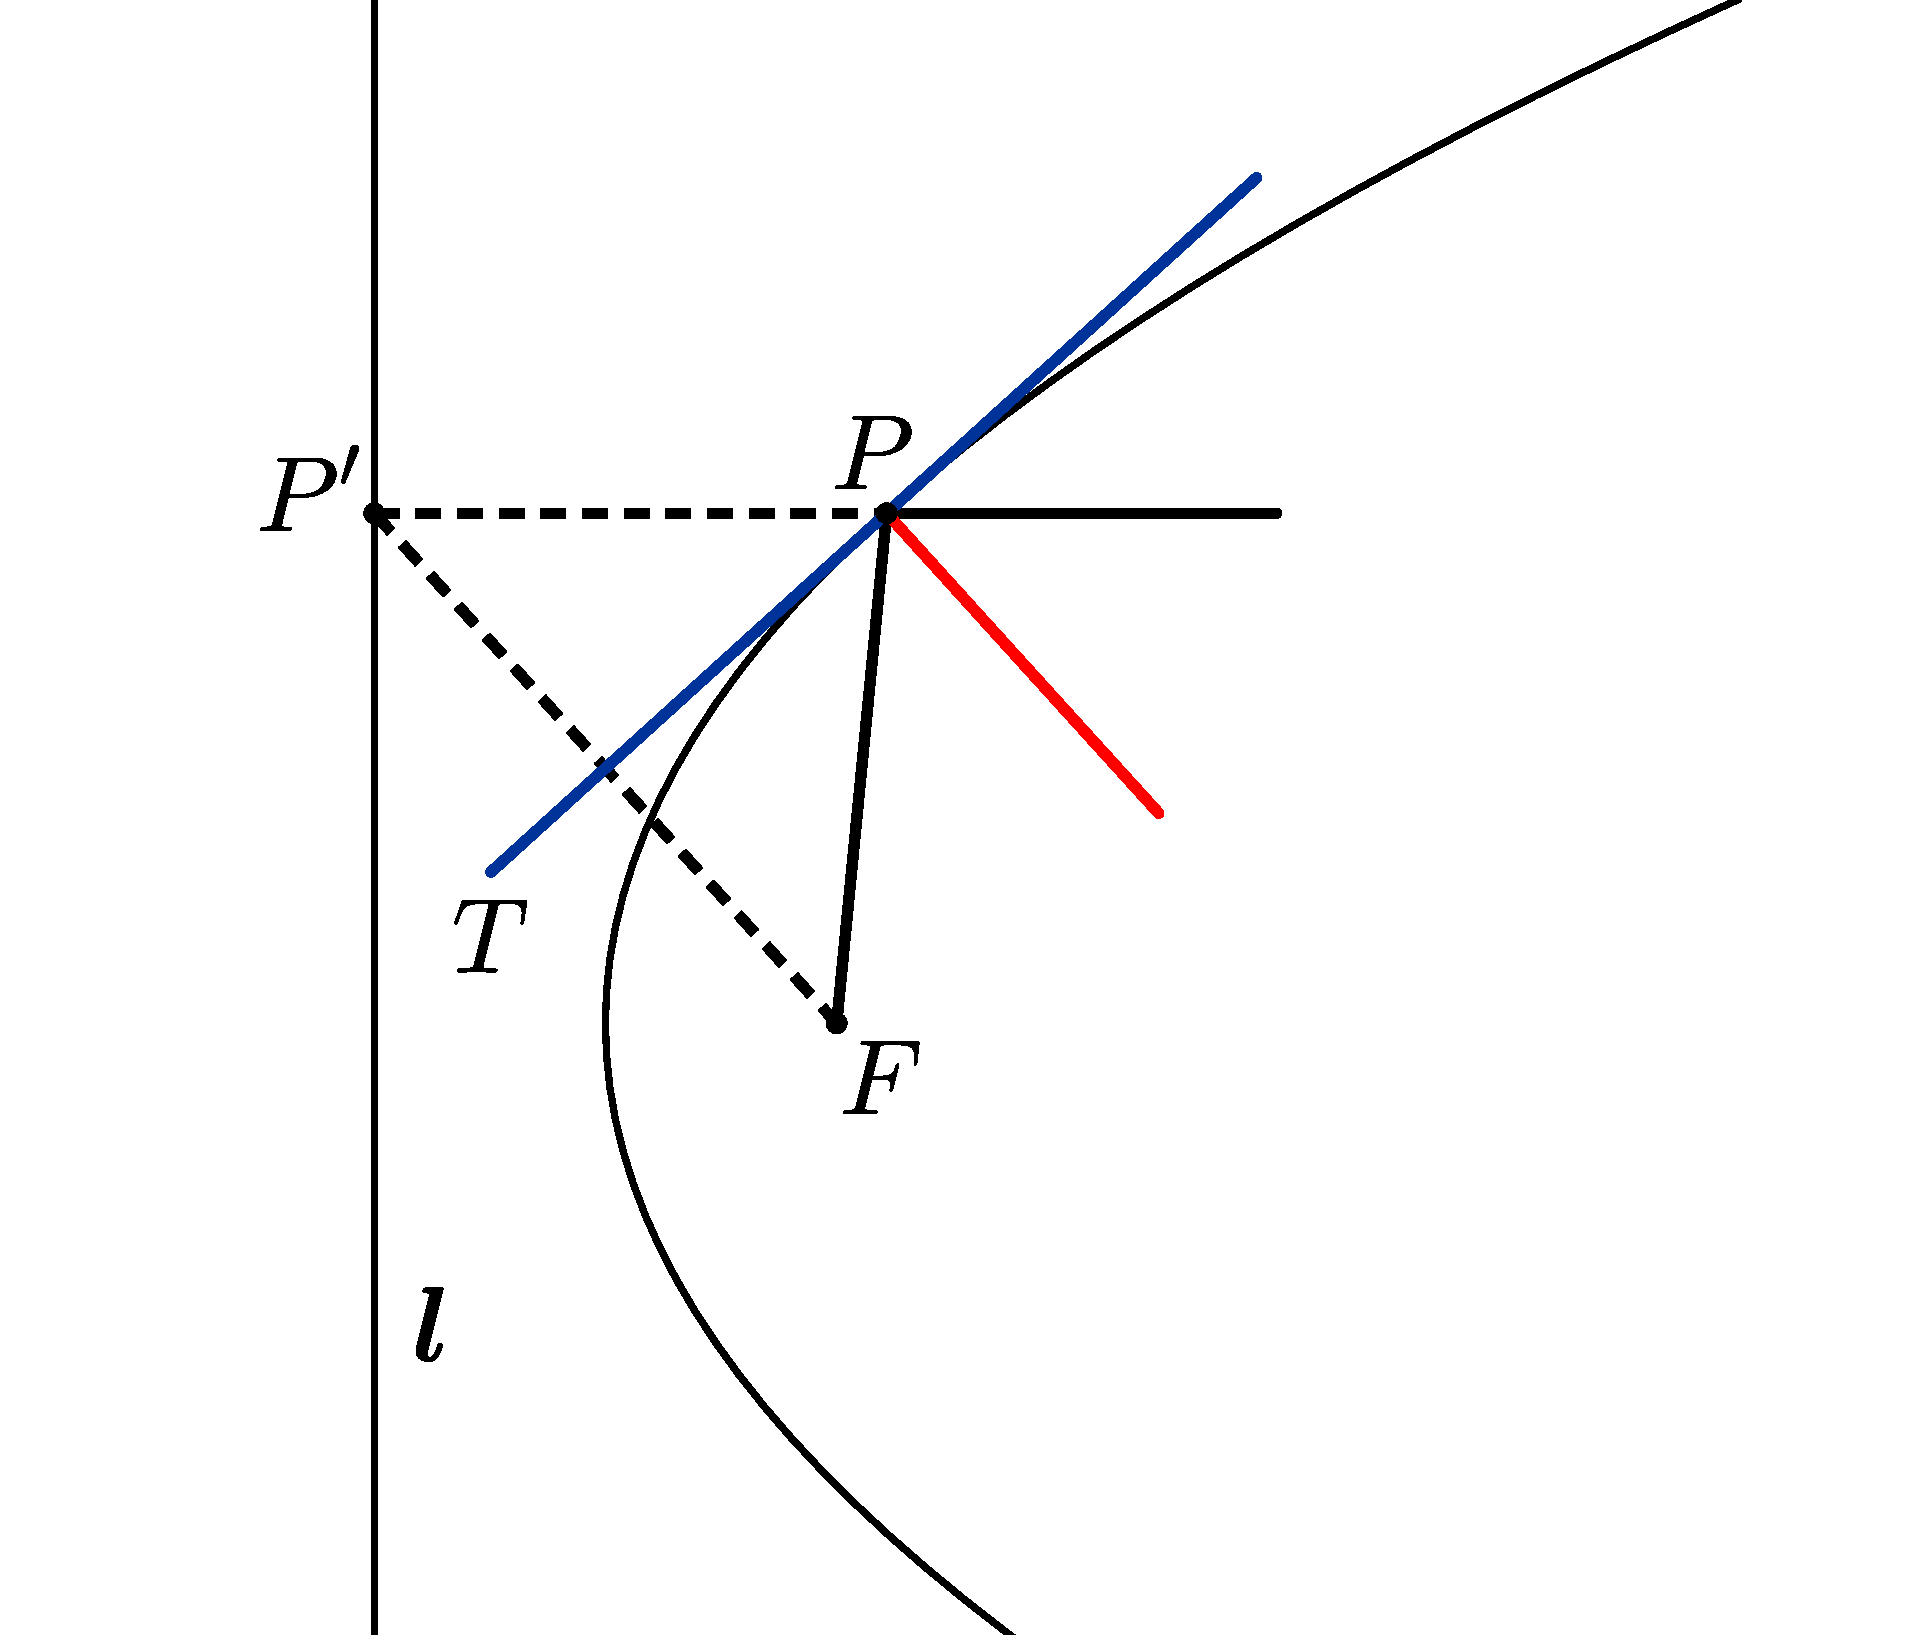
\includegraphics[width=6cm]{./figures/ConOpt4.pdf}
\caption{抛物线的光学性质} \label{ConOpt_fig4}
\end{figure}

\subsection{双曲线的光学性质}
$F_1$,$F_2$ 是双曲线的两个焦点,$P$ 是双曲线上的任意一点,则 $\angle F_1PF_2 $ 的角平分线 $ PT $ 是双曲线的切线.

等价命题:真空或同种均匀介质中,从双曲线一个焦点射出的光线,经过双曲线的反射后,反射光的反向延长线汇聚于另一个焦点.
\begin{figure}[ht]
\centering
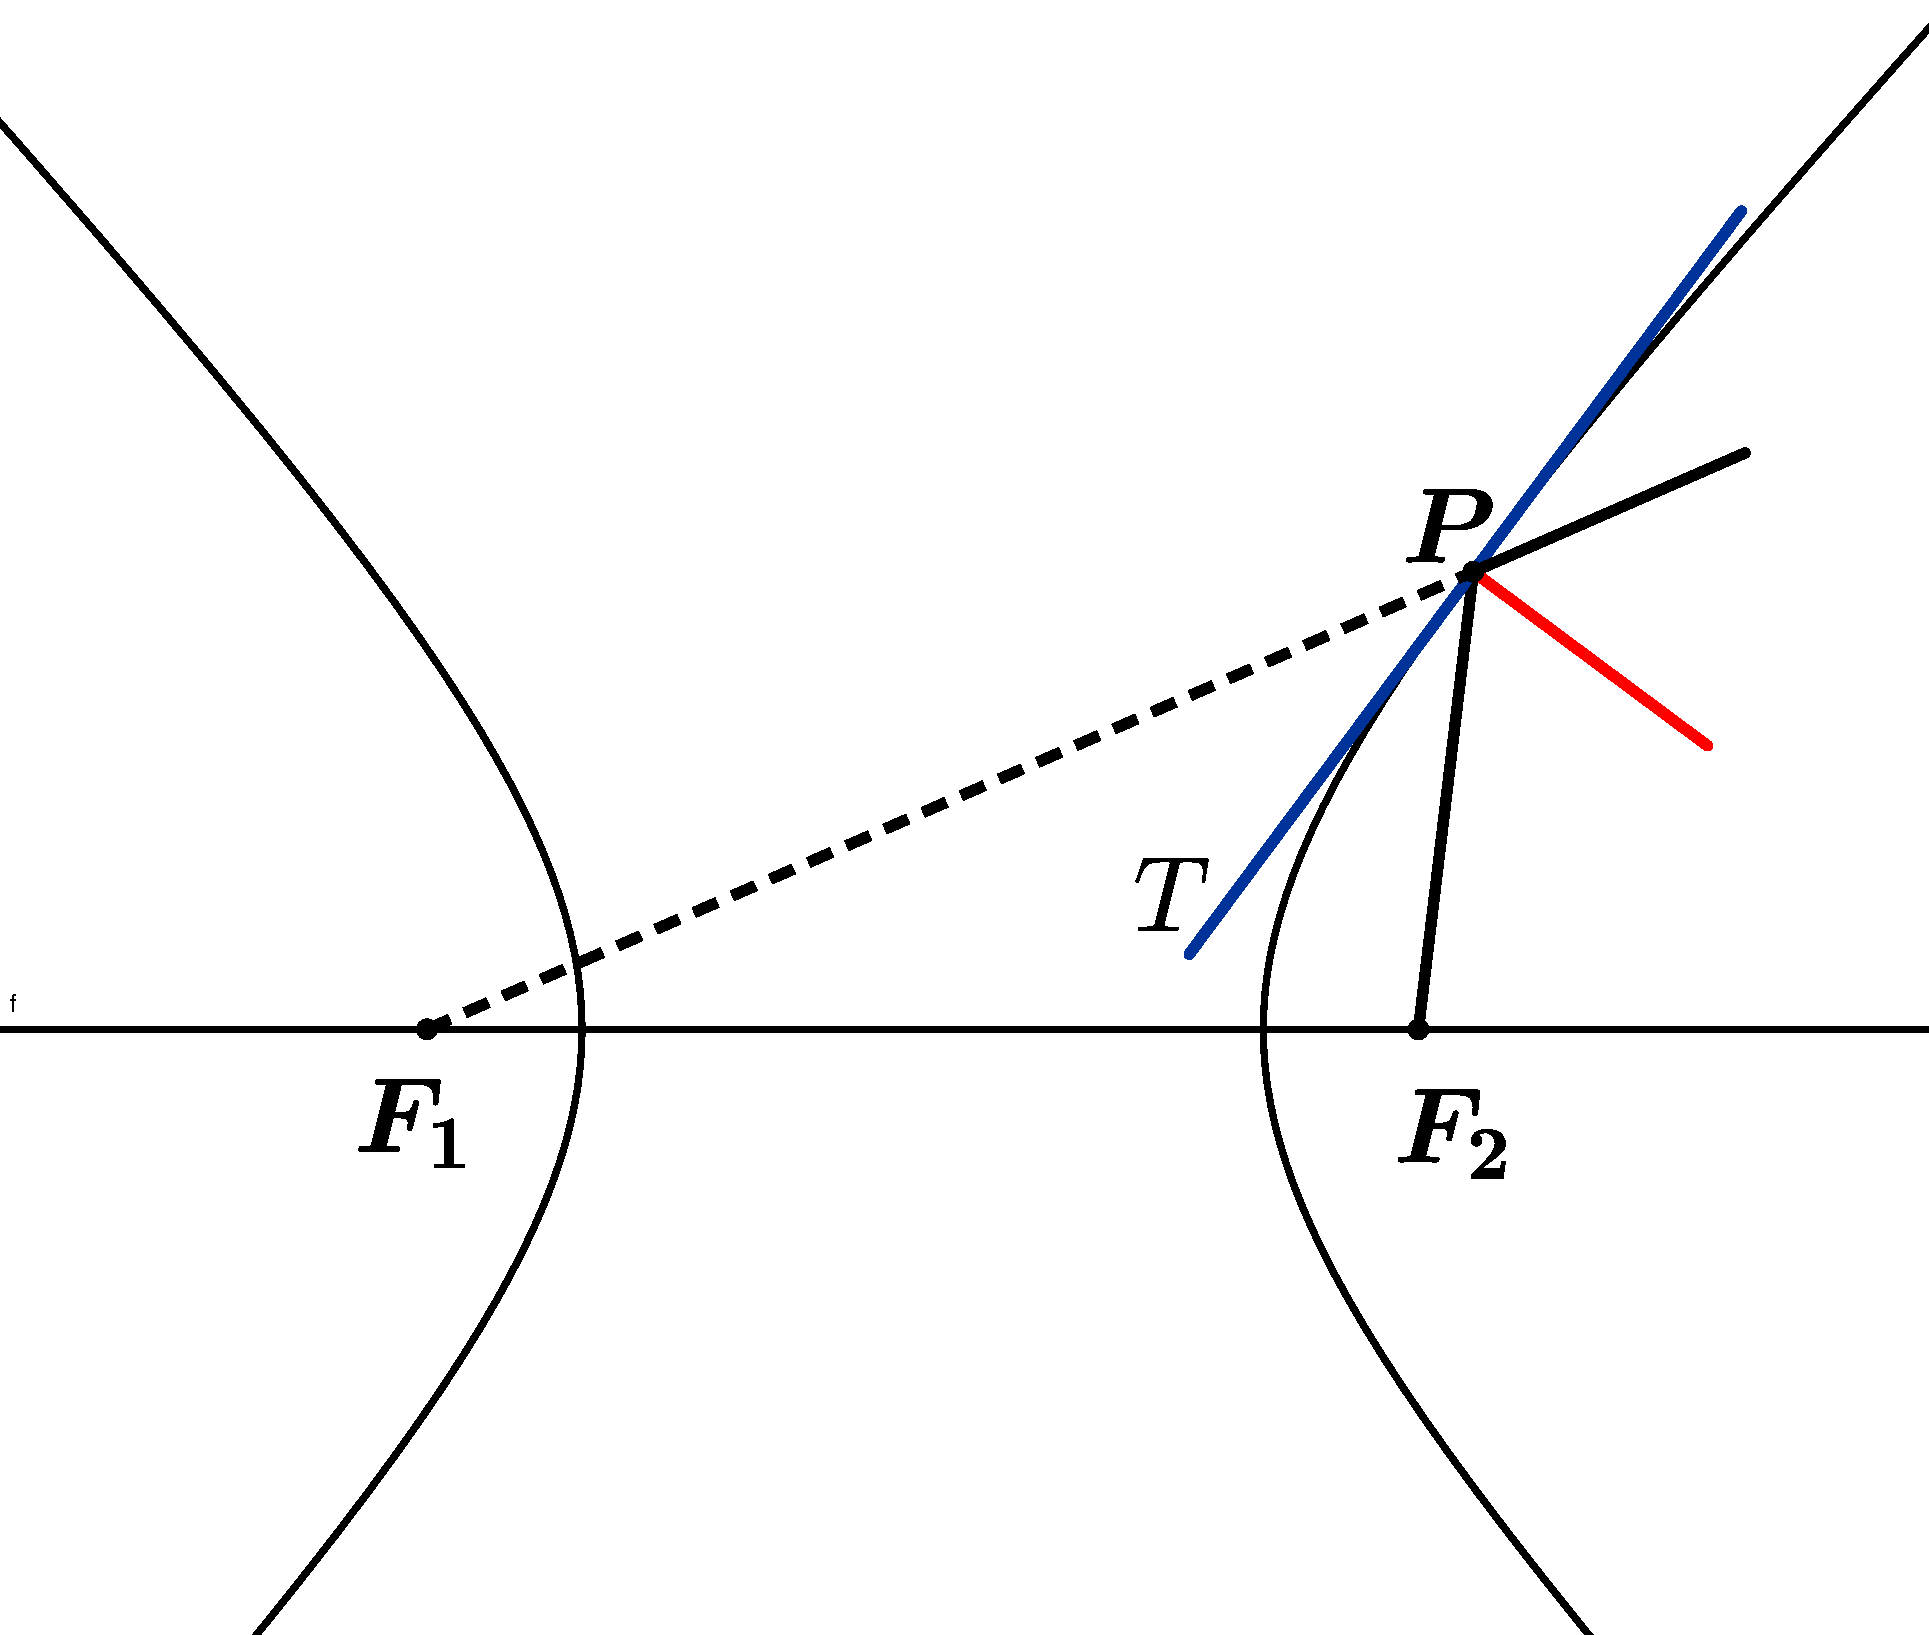
\includegraphics[width=6cm]{./figures/ConOpt5.pdf}
\caption{双曲线的光学性质} \label{ConOpt_fig5}
\end{figure}

\begin{exer}{证明题}\label{ConOpt_exe1}
仿照椭圆光学性质的证明和推导过程,证明抛物线和双曲线的光学性质.
\end{exer}
